\documentclass[border=1mm]{standalone}
\usepackage{tikz}
\usetikzlibrary{shadows,arrows.meta,positioning,calc,patterns, shapes}
\definecolor{darkgreen}{RGB}{27,114,30}

\begin{document}
  \begin{tikzpicture}[scale=1]

    % Part 1: A physical image of the CCD, with gate 12
    \node(scope1){
      \begin{tikzpicture} 
        \draw[thick] (0,0) rectangle (1.5,3); % box
        \draw[thick,blue] (0.53,-0.2) -- (0.53,3.2); % Line for gate 12
        \draw[thick,red] (1.5,0) -- (1.5,3); % Readout
        \draw[thick,-{Latex[length=8pt]}] (0.6,1.5) to (1.4,1.5);
        
        \node[blue] at (0.3,3.4) {Gate 12}; % Marker for gate 12
        \node[red] at (1.8,-0.3) {Readout}; % Marker for Readout
        \node at (1,1.8) {TDI}; % Marker for Readout


      \end{tikzpicture} 
    };

    % Part 2: The output image
    \node[at={($(scope1.east)+(.1cm,0)$)},anchor=west](scope2){
      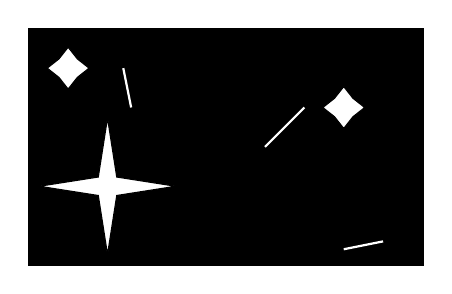
\begin{tikzpicture} 
        % the box around it
        \draw[thick, fill] (0,0) rectangle (5,3);

        % A few stars
        \node[star,star points=4, star point height=.7cm, draw, fill=white] at (1,1) {};
        \node[star,star points=4, star point height=.1cm, draw, fill=white] at (4,2) {};
        \node[star,star points=4, star point height=.1cm, draw, fill=white] at (.5,2.5) {};

        % And some cosmics
        \draw[thick,white] (3.5,2) -- (3,1.5) (1.2,2.5) -- (1.3,2)
                           (4,0.2) -- (4.5,0.3);
      \end{tikzpicture} 
    };

    % a big arrow between them
    \draw[red, ultra thick,-{Stealth[length=.5cm, width=.7cm]}] ($(scope1.east) + (-1cm,0)$)  to ($(scope2.west)$);
\end{tikzpicture}
\end{document}
